\documentclass{article}
\usepackage{polski}
\usepackage{blindtext}
\usepackage{amsmath}
\usepackage{mathtools}
\usepackage{graphicx} 
\usepackage{wrapfig}
\usepackage{amssymb}
\usepackage{multirow}
\usepackage[usenames,dvipsnames,svgnames,table]{xcolor}
\usepackage{float}
\usepackage[caption = false]{subfig}
\usepackage{caption}
\newcommand\tab[1][1cm]{\hspace*{#1}}
\usepackage[a4paper, left=2cm, right=2cm, top=2cm, bottom=2cm, headsep=1.2cm]{geometry}

\usepackage{titling}
\newcommand{\subtitle}[1]{%
  \posttitle{%
    \par\end{center}
    \begin{center}\large#1\end{center}
    \vskip0.5em}%
}


\begin{document}
\title{Całkowanie numeryczne metodą Simpsona}
\author{Wiktoria Zaczyk}
\date{27.05.2020}

\maketitle

\begin{figure}[H]
\begin{center}

\includegraphics[height=0.3\linewidth]{agh.jpg}
\label{pierwszy} 
\end{center}
\end{figure}

\section{Wstęp teoretyczny}
\textbf{Całkowanie numeryczne}
\newline
Oznacza zastosowanie metod numerycznych w celu wyznaczenia przybliżonej wartości całki oznaczonej.Proste metody całkowania numerycznego polegają na przybliżeniu całki za pomocą odpowiedniej sumy ważonej wartości całkowanej funkcji w kilku punktach. Aby uzyskać dokładniejsze przybliżenie dzieli się przedział całkowania na niewielkie fragmenty. Ostateczny wynik jest sumą oszacowań całek w poszczególnych podprzedziałach.

\begin{equation}
\begin{array}{c}
C = \displaystyle \int_{a}^{b} f(x)dx 
\end{array}
\end{equation}

\newline
\setlength{\parindent}{0pt}
\textbf{Kwadratury Newtona-Cotesa}
\newline
Rozważamy przypadek z węzłami równoodległymi $x_i=a+i\cdot h$,  $i=0,1,2,...,N$. Jeśli końce przedziału są również węzłami wówczas
kwardatury noszą nazwę kwadratur zamkniętych. Przybliżamy funkcję podcałkową
wielomianem Lagrange'a stopnia conajwyżej N:

\begin{equation}
\begin{array}{c}
f(x_i)=\displaystyle L_N(x_i), i=1,2,...,N
\end{array}
\end{equation}

\begin{equation}
\begin{array}{c}
L_N(x)=\displaystyle \sum^N_{k=0} f(x_k)\Phi_k(x)
\end{array}
\end{equation}

\begin{equation}
\begin{array}{c}
\Phi_k(x)=\displaystyle \prod_{j=0 j\ne k}\frac{x-x_j}{k_k-x_j}
\end{array}
\end{equation}

Numerycznie całkę policzyć można z następującego wzoru:

\begin{equation}
\begin{array}{c}
S(f)=\displaystyle \sum_{k=0 j}^N A_kf(x_k), \hspace{10} x\in[a,b]
\end{array}
\end{equation}

Współczynnik Ak wyraża się następującym wzorem:

\begin{equation}
\begin{array}{c}
A_k=\displaystyle h\frac{(-1)^{N-k}}{k!(N-k)!} \int_{0}^{N} \frac{t(t-1)...(t-N)}{t-k}
\end{array}
\end{equation}

\newline\newline
\setlength{\parindent}{0pt}
\textbf{Metoda Simpsona}
\newline
jest numeryczną metodą pozwalającą na obliczenie całek. W tej metodzie funkcja
podcałkowa jest przybliżana parabolą rozpiętą na krańcach przedziału całkowania oraz jego środku.

\begin{figure}[H]
\begin{center}
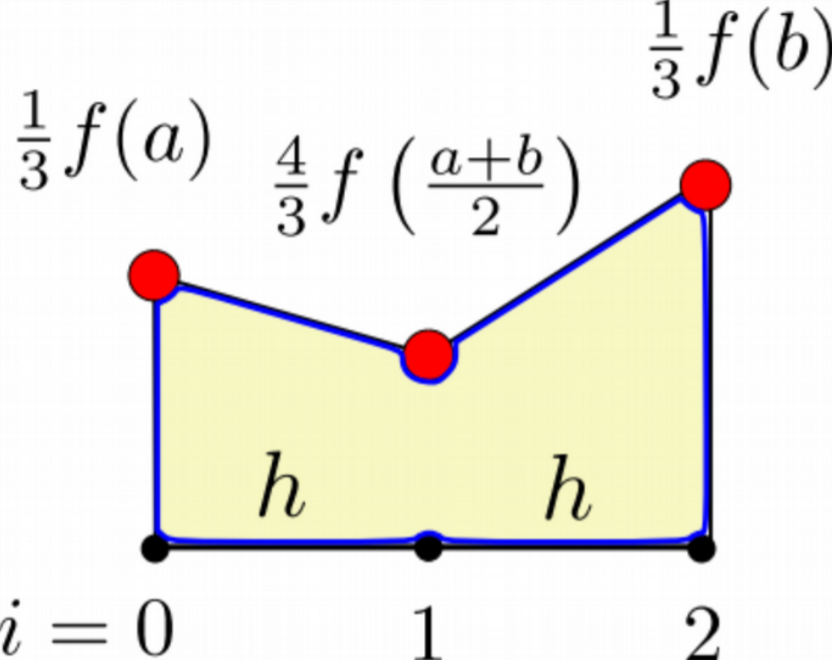
\includegraphics[height=0.3\linewidth]{wzor.png}
\label{pierwszy} 
\end{center}
\end{figure}
Przedział całkowania [a, b] dzielimy na m podprzedziałów (m jest parzyste). W podprzedziałach
[a, a+2h], . . . , [a+(m-1)h ,b] stosuje się wzór parabol a wyniki cząstkowe sumuje:

\begin{equation}
\begin{array}{c}
S(f)=\displaystyle \frac{h}{3} \sum^{m/2}_{k=1}(f_{2k-2}+4f_{2k-1}+f_2_k)
\end{array}
\end{equation}

Błąd jest równy:

\begin{equation}
\begin{array}{c}
E(f)=\displaystyle -\frac{1}{90} h^5f^{(4)}(\xi)
\end{array}
\end{equation}

\section{Cel zadania}

Zadaniem w trakcie laboratoriów było za pomocą metody Simpsona, obliczyć numerycznie całki typu: I=$\int_{0}^{\pi}x^msin(kx)dx $
Wartość dokładną obliczyliśmy rozwijając w szereg dla 30 pierwszych wyrazów. Policzyliśmy wartości dla 3 przypadków:
\begin{enumerate}
\item $m=0, k=1$
\item $m=1, k=1$
\item $m=5, k=5$
\end{enumerate}
Wartości całki liczone metodą Simpsona wyznaczyliśmy dla następującej liczby węzłów: $n=2p+1=11,21,51,101,201$

\newline
\setlength{\parindent}{0pt}
Funkcja w postaci szergu:

\begin{equation}
\begin{array}{c}
I=\displaystyle \sum^{\infty}_{i=0}(-1)^i \frac{(k x)^{2i+m+2}}{k^{m+1}(2i+1)!(2i+m+2)} \Big|^b_a
\end{array}
\end{equation}

\newpage
\section{Wyniki}
\textbf{I.  Wartość całki obliczone metodą rozwinięcia funkcji podcałkowej w szereg}

\newline
a)$m=0$, $k=1$
\begin{table}[H]
\centering
\begin{tabular}{|c|c|c|}
n& wartość całki & $|C−I|$ \\
\hline
1 & 4.9348 & 2.9348\\
2 & 0.87609 & 1.12391\\
3 & 2.21135 & 0.211353\\
4 & 1.97602 & 0.0239778\\
5 & 2.00183 & 0.0018291\\
6 & 1.9999 & 0.00010047\\
7 & 2 & 4.16781e-06\\
8 & 2 & 1.3526e-07\\
9 & 2 & 3.52908e-09\\
10 & 2 & 7.56506e-11\\
11 & 2 & 1.35669e-12\\
12 & 2 & 2.02061e-14\\
13 & 2 & 8.88178e-16\\
14 & 2 & 4.44089e-16\\
15 & 2 & 4.44089e-16\\
16 & 2 & 4.44089e-16\\
17 & 2 & 4.44089e-16\\
18 & 2 & 4.44089e-16\\
19 & 2 & 4.44089e-16\\
20 & 2 & 4.44089e-16\\
21 & 2 & 4.44089e-16\\
22 & 2 & 4.44089e-16\\
23 & 2 & 4.44089e-16\\
24 & 2 & 4.44089e-16\\
25 & 2 & 4.44089e-16\\
26 & 2 & 4.44089e-16\\
27 & 2 & 4.44089e-16\\
28 & 2 & 4.44089e-16\\
29 & 2 & 4.44089e-16\\
30 & 2 & 4.44089e-16
\end{tabular}
\caption{Wartości sum szeregu}
\end{table}
Po dodaniu 8 elementów wartość sumy szeregu zaczęła być bardzo bliska oczekiwaniu teoretycznemu.

\newpage
b)$m=1$, $k=1$
\begin{table}[H]
\centering
\begin{tabular}{|c|c|c|}
n& wartość całki & $|C−I|$ \\
\hline
1 & 10.3354 & 7.19383\\
2 & 0.134769 & 3.00682\\
3 & 3.73036 & 0.588764\\
4 & 3.07319 & 0.0684032\\
5 & 3.14689 & 0.00530114\\
6 & 3.1413 & 0.000294494\\
7 & 3.1416 & 1.23208e-05\\
8 & 3.14159 & 4.02514e-07\\
9 & 3.14159 & 1.0558e-08\\
10 & 3.14159 & 2.27316e-10\\
11 & 3.14159 & 4.09006e-12\\
12 & 3.14159 & 6.26166e-14\\
13 & 3.14159 & 4.44089e-16\\
14 & 3.14159 & 4.44089e-16\\
15 & 3.14159 & 4.44089e-16\\
16 & 3.14159 & 4.44089e-16\\
17 & 3.14159 & 4.44089e-16\\
18 & 3.14159 & 4.44089e-16\\
19 & 3.14159 & 4.44089e-16\\
20 & 3.14159 & 4.44089e-16\\
21 & 3.14159 & 4.44089e-16\\
22 & 3.14159 & 4.44089e-16\\
23 & 3.14159 & 4.44089e-16\\
24 & 3.14159 & 4.44089e-16\\
25 & 3.14159 & 4.44089e-16\\
26 & 3.14159 & 4.44089e-16\\
27 & 3.14159 & 4.44089e-16\\
28 & 3.14159 & 4.44089e-16\\
29 & 3.14159 & 4.44089e-16\\
30 & 3.14159 & 4.44089e-16

\end{tabular}
\caption{Wartości sum szeregu}
\end{table}
Po dodaniu 8 elementów wartość sumy szeregu zaczęła być bardzo bliska oczekiwaniu teoretycznemu.

\newpage
c)$m=5$, $k=5$
\begin{table}[H]
\centering
\begin{tabular}{|c|c|c|}
n& wartość całki & $|C−I|$ \\
\hline
1 & 2157.35 & 2100.99\\
2 & -66845.2 & 66901.6\\
3 & 629661 & 629604\\
4 & -2.83264e+06 & 2.83269e+06\\
5 & 7.45046e+06 & 7.4504e+06\\
6 & -1.29018e+07 & 1.29019e+07\\
7 & 1.59002e+07 & 1.59002e+07\\
8 & -1.47179e+07 & 1.47179e+07\\
9 & 1.06416e+07 & 1.06416e+07\\
10 & -6.19063e+06 & 6.19068e+06\\
11 & 2.96544e+06 & 2.96539e+06\\
12 & -1.1914e+06 & 1.19146e+06\\
13 & 407744 & 407688\\
14 & -120262 & 120318\\
15 & 31013.5 & 30957.2\\
16 & -6952.2 & 7008.56\\
17 & 1463.78 & 1407.42\\
18 & -196.104 & 252.468\\
19 & 97.0724 & 40.7088\\
20 & 50.4304 & 5.93318\\
21 & 57.1491 & 0.785554\\
22 & 56.2687 & 0.0949094\\
23 & 56.3741 & 0.0105079\\
24 & 56.3625 & 0.00106895\\
25 & 56.3637 & 0.000101369\\
26 & 56.3636 & 7.89865e-06\\
27 & 56.3636 & 1.55232e-06\\
28 & 56.3636 & 7.929e-07\\
29 & 56.3636 & 8.4974e-07\\
30 & 56.3636 & 8.45767e-07
\end{tabular}
\caption{Wartości sum szeregu}
\end{table}
Po zsumowania pierwszych 30 wyrazów wyznaczone wartości z rozwiązaniem dokładnym nie przestała
się zmieniać, jednak można zaobserwować, że po zsumowaniu 26 wyrazów była ona już bardzo niewielka. 

\newpage
\textbf{II.  Wartość całki obliczone metodą Simpsona}
\newline
a)$m=0$, $k=1$

\begin{table}[H]
\centering
\begin{tabular}{|c|c|c|}
n& wartość całki &  $|C−I|$  \\
\hline
11 & 2.000007 & 6.78444e-06\\ 
21 & 2.0 & 4.23093e-07\\ 
51  & 2.0 & 1.08245e-08\\ 
101  & 2.0 & 6.76472e-10\\ 
201  & 2.0 & 4.22777e-11
\end{tabular}
\caption{Wartości całki obliczone metodą Simpsona}
\end{table}

\begin{figure}[H]
\begin{center}
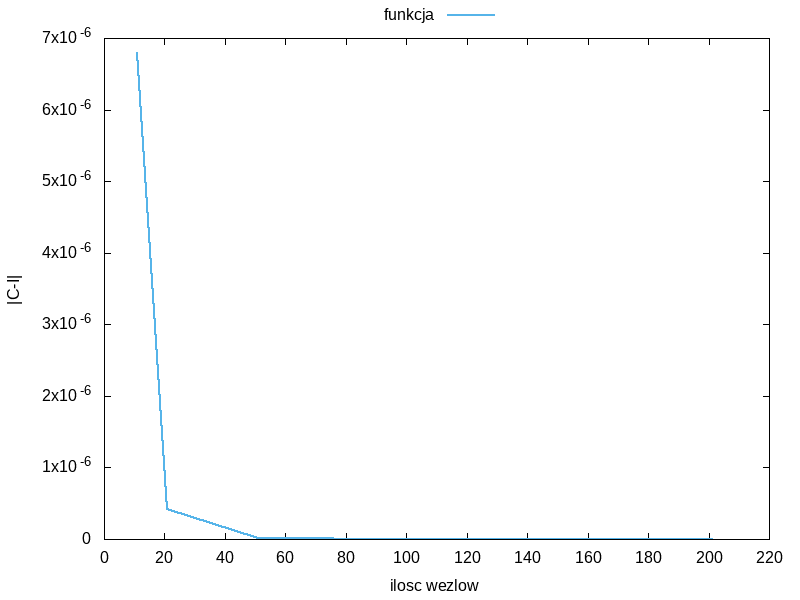
\includegraphics[height=0.5\linewidth]{2a.jpg}
\caption{Wykres zależności różnicy wartości dokładnej całki, a całki obliczonej numerycznie od ilości przyjętych
węzłów}
\label{pierwszy} 
\end{center}
\end{figure}

b)$m=1$, $k=1$

\begin{table}[H]
\centering
\begin{tabular}{|c|c|c|}
n& wartość całki &  $|C−I|$  \\
\hline
11 & 3.141603 & 1.0657e-05\\ 
21 & 3.141593 & 6.64593e-07\\ 
51  & 3.141593 & 1.70031e-08\\ 
101  & 3.141593 & 1.0626e-09\\ 
201  & 3.141593 & 6.64095e-11
\end{tabular}
\caption{Wartości całki obliczone metodą Simpsona}
\end{table}

\begin{figure}[H]
\begin{center}
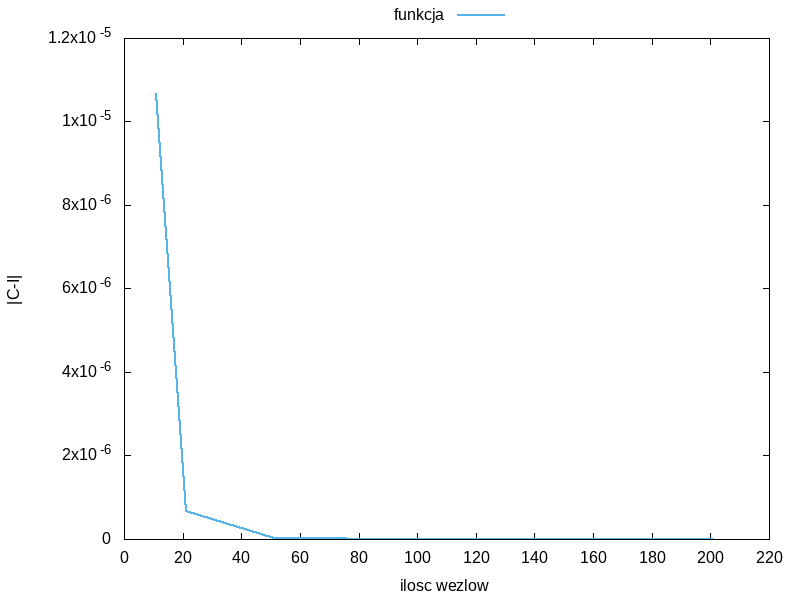
\includegraphics[height=0.5\linewidth]{2b.jpg}
\caption{Wykres zależności różnicy wartości dokładnej całki, a całki obliczonej numerycznie od ilości przyjętych
węzłów}
\label{pierwszy} 
\end{center}
\end{figure}

c)$m=5$, $k=5$

\begin{table}[H]
\centering
\begin{tabular}{|c|c|c|}
n& wartość całki &  $|C−I|$  \\
\hline
11 & 56.462920 & 0.0993507\\ 
21 & 56.369718 & 0.00614874\\ 
51  & 56.363727 & 0.000157636\\ 
101  & 56.363580 & 1.06398e-05\\ 
201  & 56.363570 &  1.45813e-06
\end{tabular}
\caption{Wartości całki obliczone metodą Simpsona}
\end{table}

\begin{figure}[H]
\begin{center}
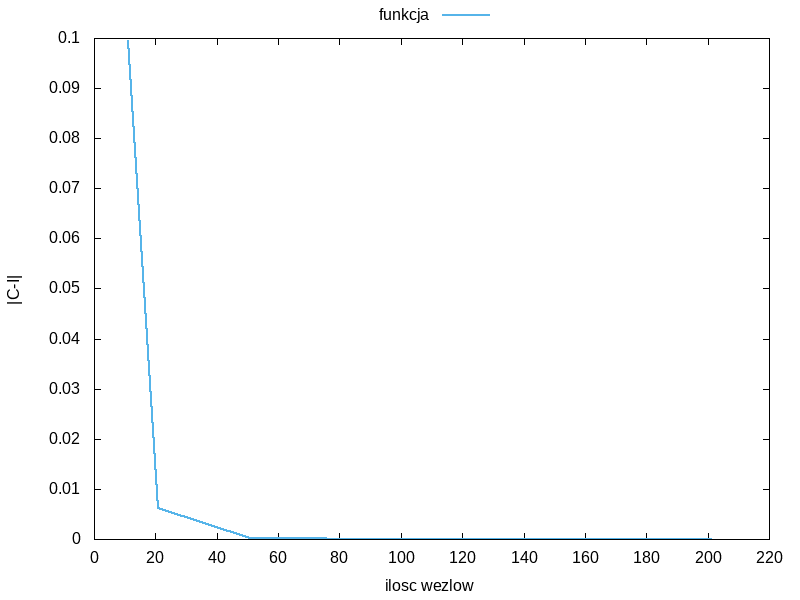
\includegraphics[height=0.5\linewidth]{2c.jpg}
\caption{Wykres zależności różnicy wartości dokładnej całki, a całki obliczonej numerycznie od ilości przyjętych
węzłów}
\label{pierwszy} 
\end{center}
\end{figure}



\section{Wnioski}
Przy rozwijaniu funkcji w szereg dla kolejnych iteracji funkcja zmierza do punktu zbieżności. Dla małej liczby iteracji widać zaburzenia. Przy korzystaniu z metody Simpsona dla liczby wezłów: $m=0$, $k=1$ wartość całki jest bardzo dokładna, w pozostałych przypadkach wartości całki są bardzo bliskie. Wraz ze wzrostem liczby węzłów, zwiększała się dokładność przybliżenia. Metoda Simpsona okazała się być skuteczną i szybką metodą do numerycznego obliczenia wartości całki oznaczonej. Podobnie jak dla metoda interpolacji.

\begin{thebibliography}{1}

\bibitem{1}
	Tomasz Chwiej, \emph{Szybka transformacja Fouriera} \\
	\texttt{http://galaxy.agh.edu.pl/$\sim$chwiej/mn/calkowanie\_1819.pdf}	
\bibitem{2}	
	\texttt{https://pl.wikipedia.org/wiki/Całkowanie\_numeryczne}
	

\end{thebibliography}

\end{document}